% Created by Takeuchi on Aug. 2020
\documentclass[dvipdfmx, 11pt]{beamer}

%%%% Packages %%%%%
%\usepackage{bxdpx-beamer}
%\usepackage{minijs}
%\usepackage{otf}
%\usepackage{tabularx}
%\usepackage{graphicx}
% \usepackage{graphicx}
% \usepackage{amsmath,amssymb,amsthm}
% \usepackage{multirow}
\usepackage{multicol}
% \usepackage{url}
\usepackage{tikz}
\usetikzlibrary{arrows,shapes}
\usetikzlibrary{positioning}
% \usepackage{alltt}
% \usepackage{bm}
 \usepackage{listings,jlisting}
% \usepackage{listings}
% \lstset{
%  basicstyle=\ttfamily\scriptsize,
%  keepspaces=true,
%  escapechar=|,
%  columns=[l]{fullflexible}
% }

%%%% Fonts %%%%%
\renewcommand{\kanjifamilydefault}{\gtdefault}
 %\usepackage{otf} % otfパッケージ
 \usepackage[deluxe]{otf} 
%\renewcommand{\kanjifamilydefault}{mg}
\usepackage{txfonts} % 数式・英文ローマン体を Lxfont にする
% \usepackage[T1]{fontenc} % 8bit フォント
% \usepackage{minijs}
% \usepackage{textcomp} % 欧文フォントの追加
% \usepackage[utf8]{inputenc} % 文字コードをUTF-8

%%%%% Beamer %%%%%
\usetheme{Madrid}
\useinnertheme{rectangles}
%\useoutertheme{smoothbars}
\setbeamercolor{enumerate}{fg=white, bg=black}
\usefonttheme{professionalfonts}
\setbeamertemplate{frametitle}[default][center]
\setbeamertemplate{navigation symbols}{}
% \setbeamercovered{transparent} % 好みに応じてどうぞ
\setbeamertemplate{footline}[frame number]
\setbeamercolor{page number in head/foot}{fg=black} % ページ数を表示する
% \setbeamerfont{footline}{size=\normalsize,series=\bfseries}
\setbeamerfont{footline}{size=\scriptsize,series=\mdseries}
\setbeamercolor{footline}{fg=black,bg=black}
\setbeamertemplate{blocks}[rounded][shadow=true]
\setbeamertemplate{items}[ball]
% \setbeamertemplate{enumerate items}[default]
% \setbeamerfont{alerted text}{series=\bfseries}
\newcommand{\backupbegin}{
   \newcounter{framenumberappendix}
   \setcounter{framenumberappendix}{\value{framenumber}}
}
\newcommand{\backupend}{
   \addtocounter{framenumberappendix}{-\value{framenumber}}
   \addtocounter{framenumber}{\value{framenumberappendix}} 
}
\renewcommand{\thefootnote}{\dag} % フットノート番号をダガーにする

%%%% Code %%%%%%%%%
\lstset{
 basicstyle=\ttfamily\color{black},
 keepspaces=true,
 escapechar=|,
 columns=[l]{fullflexible},
 commentstyle={\color{red}},
 stringstyle={\color{blue}},
 % literrate =%
 %   {:-}{{\textcolor{black}{:-}}}2%
 %   {,}{{\textcolor{black}{,}}}1%
 %   {.}{{\textcolor{black}{.}}}1%
}

%%%% My macro %%%%%
%%%%%%%%%%%%%%%%%%%%%%%%%%%%%%%%%%%%%%%%%%%%%%%%%%%%%%%%%%%%%%%%
% User-defined Macro
%%%%%%%%%%%%%%%%%%%%%%%%%%%%%%%%%%%%%%%%%%%%%%%%%%%%%%%%%%%%%%%%
\newcommand{\compress}{\itemsep0pt\parsep0pt\parskip0pt\partopsep0pt}
% \newcommand{\compress}{\itemsep1pt plus1pt\parsep0pt\parskip0pt}
% \newcommand{\code}[1]{\lstinline[basicstyle=\ttfamily]{#1}}
\newcommand{\gringo}{\textit{gringo}}
\newcommand{\clasp}{\textit{clasp}}
\newcommand{\clingo}{\textit{clingo}}
\newcommand{\teaspoon}{\textit{teaspoon}}
\newcommand{\sat}{\textsf{SAT}}
\newcommand{\unsat}{\textsf{UNSAT}}
% \newcommand{\web}[2]{\href{#1}{#2\ \raisebox{-0.15ex}{\beamergotobutton{Web}}}}
% \newcommand{\doi}[2]{\href{#1}{#2\ \raisebox{-0.15ex}{\beamergotobutton{DOI}}}}
% \newcommand{\weblink}[1]{\web{#1}{#1}}
% \newcommand{\imp}{\mathrel{\Rightarrow}}
% \newcommand{\Iff}{\mathrel{\Leftrightarrow}}
% \newcommand{\mybox}[1]{\fbox{\rule[.2cm]{0cm}{0cm}\mbox{${#1}$}}}
% \newcommand{\mycbox}[2]{\tikz[baseline]\node[fill=#1!10,anchor=base,rounded corners=2pt] () {#2};}
% \newcommand{\naf}[1]{\ensuremath{{\sim\!\!{#1}}}}
% \newcommand{\head}[1]{\ensuremath{\mathit{head}(#1)}}
% \newcommand{\body}[1]{\ensuremath{\mathit{body}(#1)}}
% \newcommand{\atom}[1]{\ensuremath{\mathit{atom}(#1)}}
% \newcommand{\poslits}[1]{\ensuremath{{#1}^+}}
% \newcommand{\neglits}[1]{\ensuremath{{#1}^-}}
% \newcommand{\pbody}[1]{\poslits{\body{#1}}}
% \newcommand{\nbody}[1]{\neglits{\body{#1}}}
% \newcommand{\Cn}[1]{\ensuremath{\mathit{Cn}(#1)}}
% \newcommand{\reduct}[2]{\ensuremath{#1^{#2}}}
% \newcommand{\OK}{\mbox{\textcolor{green}{\Pisymbol{pzd}{52}}}}
% \newcommand{\KO}{\mbox{\textcolor{red}{\Pisymbol{pzd}{56}}}}
% \newcommand{\code}[1]{\lstinline[basicstyle=\ttfamily]{#1}}
% \newcommand{\lw}[1]{\smash{\lower2.ex\hbox{#1}}}
\newcommand{\llw}[1]{\smash{\lower3.ex\hbox{#1}}}

\newenvironment{tableC}{%
  \scriptsize
  \renewcommand{\arraystretch}{0.9}
  \tabcolsep = 0.6mm
  % \begin{tabular}[t]{p{6mm}|rlr|rlr|rlr|rlr|rlr}\hline
  %   \multicolumn{1}{l|}{\llw{問題   }} &
  \begin{tabular}[t]{l|rlr|rlr|rlr|rlr|rlr}\hline
    \multicolumn{1}{l|}{\llw{問題}} &
    \multicolumn{3}{c|}{UD1} &
    \multicolumn{3}{c|}{UD2} &
    \multicolumn{3}{c|}{UD3} &
    \multicolumn{3}{c|}{UD4} &
    \multicolumn{3}{c}{UD5} \\
    & 
    \multicolumn{1}{c}{既知の} & & \multicolumn{1}{c|}{ASP} & 
    \multicolumn{1}{c}{既知の} & & \multicolumn{1}{c|}{ASP} & 
    \multicolumn{1}{c}{既知の} & & \multicolumn{1}{c|}{ASP} & 
    \multicolumn{1}{c}{既知の} & & \multicolumn{1}{c|}{ASP} & 
    \multicolumn{1}{c}{既知の} & & \multicolumn{1}{c}{ASP} \\
    & 
    ベスト & &  & 
    ベスト & &  & 
    ベスト & &  & 
    ベスト & &  & 
    ベスト & &  \\
    \hline
  }{%
    \hline
  \end{tabular}
}

\newcommand{\nodeVP}[3]{
  \coordinate[#2] (#1);
  \draw[fill=cyan!30] (#1)--+(-1,0)--+(0,1)--+(1,0)--cycle;
  \draw (#1)node[above]{\tiny{#3}};
  \draw[fill=black] (#1) +(-0.5,0.5)--+(0.5,0.5)--+(0,1)--cycle;
  \node[rectangle,above=0.5cm of #1,white](vp){\tiny{VP}};
  \coordinate[below=0.5cm of #1] (via_#1);
  \draw (via_#1)node[above right]{\tiny{[1..1]}};
  \draw (via_#1) +(170:0.2) arc (170:370:0.2);
  \draw (#1)--(via_#1);

}
\newcommand{\nodeTrans}[3]{
  \coordinate[#2] (#1);
  \draw[fill=cyan!30] (#1)--+(-1,0)--+(0,1)--+(1,0)--cycle;
  \draw (#1)node[above]{\tiny{#3}};
  \draw[fill=black] (#1) +(-0.5,0.5)--+(0.5,0.5)--+(0,1)--cycle;
  \node[rectangle,above=0.5cm of #1,white](vp){\tiny{VP}};
  \coordinate[below=1.7cm of #1] (via_#1);
  \draw (via_#1)node[below=0.2cm]{\tiny{[1..1]}};
  \draw (via_#1) +(135:0.2) arc (135:405:0.2);
  \draw (#1)--(via_#1);

}

\newcommand{\nodeVPdashed}[3]{
  \coordinate[#2] (#1);
  \draw[fill=cyan!30,dashed] (#1)--+(-1,0)--+(0,1)--+(1,0)--cycle;
  \draw (#1)node[above]{\tiny{#3}};
  \fill[black] (#1) +(-0.5,0.5)--+(0.5,0.5)-- +(0,1)--cycle;
  \node[rectangle,above=0.5cm of #1,white](vp){\tiny{VP}};
  \coordinate[below=0.5cm of #1] (via_#1);
  \draw (via_#1)node[above right]{\tiny{[1..1]}};
  \draw (via_#1) +(-0.2,0) arc (180:360:0.2);
  \draw (#1)--(via_#1);

}

\newcommand{\nodeV}[4]{
  \node [draw,inner xsep=2pt,#2,fill=black!10,font=\tiny] (#1){
      \begin{tabular}{l}
       #3\\
       #4\\
      \end{tabular}
  };
  \fill [black] (#1.north west)--++(0,-2mm)--++(1mm,0)--++(1mm,0)--++(0,2mm); 
  \draw (#1.north west) ++(1mm,-1mm) node[white]{\tiny{v}};
}

\newcommand{\nodeVchoiced}[4]{
  \node [draw,inner xsep=2pt,#2,fill=red!50,font=\tiny] (#1){
      \begin{tabular}{l}
       #3\\
       #4\\
      \end{tabular}
  };
  \fill [black] (#1.north west)--++(0,-2mm)--++(1mm,0)--++(1mm,0)--++(0,2mm); 
  \draw (#1.north west) ++(1mm,-1mm) node[white]{\tiny{v}};

}

%%%%%%%%%%%%%%%%%%%%%%%%%%%%%%%%%%%%%%%%%%%%%%%%%%%%
\title{車両装備仕様問題に対する\\解集合プログラミングの適用}
\author{竹内頼人\inst{1} \and 田村直之\inst{2} \and 番原睦則\inst{1}}
\institute{\inst{1}名古屋大学 大学院情報学研究科 \and \inst{2}神戸大学 情報基盤センター}
\date{CAFE問題に関する意見交換会(2020/10/16)}
%\date{日本ソフトウェア科学会第37回大会 (JSSST2020)}
%\date{NII共同研究 第1回会合}
\begin{document}
\frame{\titlepage}
%%%%%%%%%%%%%%%%%%%%%%%%%%%%%%%%%%%%%%%%%%%%%%%%%%%%
\begin{frame}{車両装備仕様問題}
  \begin{alertblock}{車両装備仕様とは}
    簡単に言うと,自動車のカタログに記載されている
    \textbf{モデル/グレードと装備の一覧表}のことである.
  \end{alertblock}

  \begin{itemize}
  \item 車両の装備を決定するには,販売される国や地域の法規や規制,
    地域や市場の特性,市場の嗜好や競合など十分に考慮する必要がある.
  \item 現状では,専門知識をもつ技術者の多大な労力が費やされている.
  \item 装備仕様決定の自動化・効率化は自動車メーカーにとって重要な課題
    の一つである.
  \end{itemize}

  \begin{block}{車両装備仕様問題 (組合せ最適化問題の一種)}
    \begin{itemize}
    \item 装備タイプと装備オプションに対する
      \structure{\bf 範囲制約},
      \structure{\bf 依存制約},
      \structure{\bf 燃費制約}
      から構成される.
    \item 予想販売台数が最大となる装備仕様を求めることが目的である.
    \end{itemize}
  \end{block}
\end{frame}
%%%%%%%%%%%%%%%%%%%%%%%%%%%%%%%%%%%%%%%%%%%%%%%%%%%%
\begin{frame}{CAFE基準 (企業別平均燃費基準)}
  \begin{alertblock}{CAFE 問題}\centering
    CAFE 方式と呼ばれる燃費規制に基づく車両装備仕様問題~\footnotemark
  \end{alertblock}

  \begin{itemize}
  \item CAFE 方式は,車種別ではなくメーカー全体での出荷台数を加味した
    平均燃費を算出し,規制をかける方式.
  \item $n$車種の場合,車種$i$の燃費を$FE_i$,販売台数を$SV_i$とすると,
    \[
      \begin{array}{lcr}
        \underbrace{
        \frac{\sum_{i=1}^{n} FE_{i}\cdot SV_{i}}
        {\sum_{i=1}^{n} SV_{i}}}_{\textrm{平均燃費}
        }
        &
        \geq 
        &
        \textrm{CAFE基準値($t$)}
      \end{array}
    \]
  \item ある特定の車種では燃費基準を達成できなくても,他の車種の燃費を
    向上させることで基準を達成することが可能
  \item 欧米で採用されており,日本でも2020年度の基準として初めて導入されている.
  \end{itemize}
 \footnotetext{本研究では,CAFE方式の計算方法として,単純化された式を扱っている.}
\end{frame}
%%%%%%%%%%%%%%%%%%%%%%%%%%%%%%%%%%%%%%%%%%%%%%%%%%%%
\begin{frame}{CAFE問題の例}

  \begin{columns}
    \begin{column}{0.75\linewidth}
      \scalebox{0.8}[0.8]{ 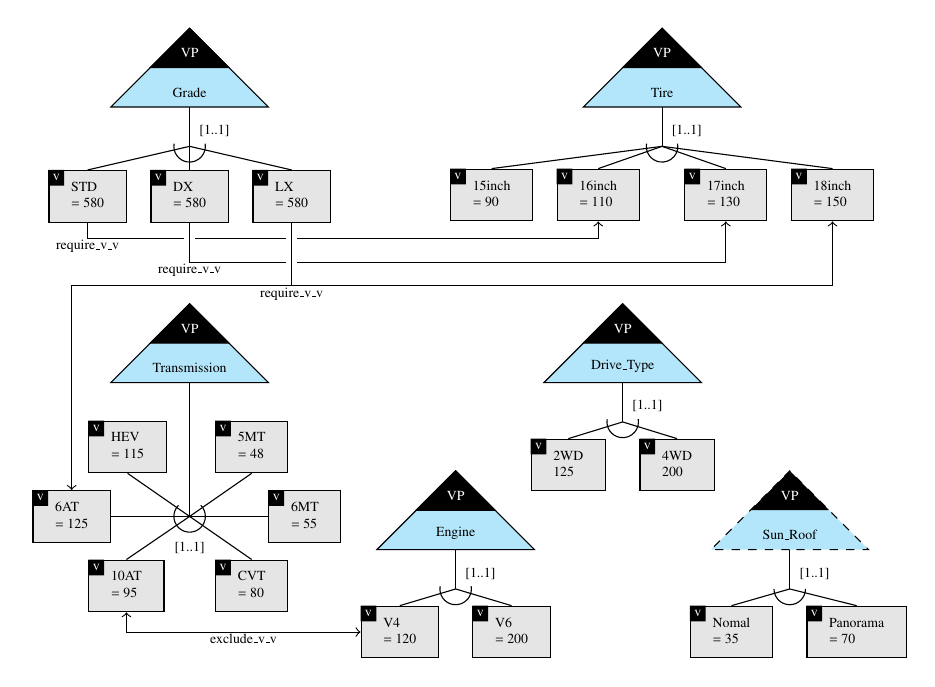
\begin{tikzpicture}
 % Grade
  \nodeVP{grade}{at={(0,0)}}{Grade};
  \nodeV{dx}{below=0.3cm of via_grade}{DX}{= 580};
  \draw(via_grade)--(dx.north);
  \nodeV{std}{left=0.3cm of dx}{STD}{= 580};
  \draw(via_grade)--(std.north);
  \nodeV{lx}{right=0.3cm of dx}{LX}{= 580};
  \draw(via_grade)--(lx.north);

  % Tire
  \nodeVP{tire}{right=6cm of grade}{Tire};
  \nodeV{16inch}{below left=0.4cm of via_tire}{16inch}{= 110};
  \nodeV{17inch}{below right=0.4cm of via_tire}{17inch}{= 130};
  \nodeV{15inch}{left=0.3cm of 16inch}{15inch}{= 90};
  \nodeV{18inch}{right=0.3cm of 17inch}{18inch}{= 150};
  \draw (via_tire)--(15inch.north);
  \draw (via_tire)--(16inch.north);
  \draw (via_tire)--(17inch.north);
  \draw (via_tire)--(18inch.north);

  % Transmission
  \nodeTrans{trans}{below=3.5cm of grade}{Transmission};
  \nodeV{6at}{left=1cm of via_trans}{6AT}{= 125};
  \nodeV{hev}{above right=0.3cm of 6at.north}{HEV}{= 115};
  \nodeV{10at}{below right=0.3cm of 6at.south}{10AT}{= 95};
  \nodeV{6mt}{right=1cm of via_trans}{6MT}{= 55};
  \nodeV{5mt}{above left=0.3cm of 6mt.north}{5MT}{= 48};
  \nodeV{cvt}{below left=0.3cm of 6mt.south}{CVT}{= 80};
  \draw (via_trans)--(10at.north);
  \draw (via_trans)--(6at.east);
  \draw (via_trans)--(hev.south);
  \draw (via_trans)--(6mt.west);
  \draw (via_trans)--(5mt.south);
  \draw (via_trans)--(cvt.north);

  % Drive_Type
  \nodeVP{drivetype}{right=5.5cm of trans}{Drive\_Type};
  \nodeV{2wd}{below left=0.3cm of via_drivetype}{2WD}{125};
  \draw (via_drivetype)--(2wd.north);
  \nodeV{4wd}{below right=0.3cm of via_drivetype}{4WD}{200};
  \draw (via_drivetype)--(4wd.north);


  % Sun_Roof
  \nodeVPdashed{sunroof}{below right=3cm of drivetype}{Sun\_Roof};
  \nodeV{nomal}{below left=0.3cm of via_sunroof}{Nomal}{= 35};
  \draw (via_sunroof)--(nomal.north);
  \nodeV{panorama}{below right=0.3cm of via_sunroof}{Panorama}{= 70};
  \draw (via_sunroof)--(panorama.north);

  % Engine
  \nodeVP{engine}{below left=3cm of drivetype}{Engine};
  \nodeV{v4}{below left=0.3cm of via_engine}{V4}{= 120};
  \draw (via_engine)--(v4.north);
  \nodeV{v6}{below right=0.3cm of via_engine}{V6}{= 200};
  \draw (via_engine)--(v6.north);
  
 

  % require
  \draw[->] (std.south)--++(0,-0.2) node[below=-1mm] {\tiny{require\_v\_v}} -|(16inch.south);
  \draw[white,line width=4pt](dx.south) ++(0,-0.1)--++(0,-0.5);
  \draw[->] (dx.south)--++(0,-0.5) node[below=-1mm] {\tiny{require\_v\_v}} -|(17inch.south);
  \draw[white,line width=4pt] (lx.south) ++(0,-0.1)--++(0,-0.8);
  \draw[->] (lx.south)--++(0,-0.8) node[below=-1mm] {\tiny{require\_v\_v}} -|(18inch.south);
  \draw[->] (lx.south)--++(0,-0.8) -|(6at.north);

  % exclude
  \draw[<->] (v4.west)-|(10at.south) node[pos=0.25,below=-1mm]{\tiny{exclude\_v\_v}};
 \end{tikzpicture}
}
      \uncover<2>{
      \begin{exampleblock}{}\centering
        STD,DX,LXグレードの3車種を生産するとする.
      \end{exampleblock}}
    \end{column}
    \begin{column}{0.25\linewidth}
      \begin{footnotesize}
        \begin{itemize}
        \item プロダクトライン開発で用いられる可変性モデルによって記述
        \item 6個の装備タイプ,19個の装備オプション
        \item 各タイプの選択可能なオプション数はすべて1
        \item 各オプションの数字は IWR 値と呼ばれ,直観的にはその重量
        \item 5個の依存制約
        \item \textsf{Sun Roof}以外は必須タイプ
        \end{itemize}
      \end{footnotesize}
    \end{column}
  \end{columns}
\end{frame}
%%%%%%%%%%%%%%%%%%%%%%%%%%%%%%%%%%%%%%%%%%%%%%%%%%%%
\begin{frame}{CAFE問題の解 {\normalsize (CAFE基準値: 9.0km/L)}}\small
 \begin{exampleblock}{解の例}
  \centering
  \renewcommand{\arraystretch}{0.9}
  %\tabcolsep = 5mm
  \begin{tabular}{p{10mm}|p{25mm}|p{15mm}|p{15mm}|p{15mm}} 
    \multicolumn{2}{l|}{装備仕様}  & 車種1 & 車種2 & 車種3 \\\hline
    装備 & \textsf{Grade}  & \textsf{STD}    & \textsf{DX}     & \textsf{LX}\\
    &\textsf{Drive\_Type}  & \textsf{2WD}    & \textsf{2WD}    & \textsf{2WD}\\
    &\textsf{Engine}	   & \textsf{V4}     & \textsf{V6}     & \textsf{V6}\\
    &\textsf{Tire}	   & \textsf{16inch} & \textsf{17inch} & \textsf{18inch}\\
    &\textsf{Transmission} & \textsf{5MT}    & \textsf{6MT}    & \textsf{10AT}\\
    &\textsf{Sun\_Roof}    & -               & \textsf{Normal} & -  
  \end{tabular}
 \end{exampleblock}
 \pause
 
 \begin{block}{}
  \centering
  \renewcommand{\arraystretch}{0.9}
  %\tabcolsep = 5mm
  \begin{tabular}{p{38mm}|p{15mm}|p{15mm}|p{15mm}} 
     IWR 値の総和 & 983  & 1,125   & 1,180 \\ %\hline
     燃費(km/L)      & 10.2  & 8.9     & 8.5 \\ %\hline
     予想販売台数    & 745   & 1,988   & 1,171  \\ \hline
     平均燃費(km/L)  & \multicolumn{3}{c}{9.0} \\ 
     予想販売台数(合計)  & \multicolumn{3}{c}{3,904} \\ 
  \end{tabular}
  \end{block}
 \vfill
 \begin{itemize}
 \item 車種2と車種3はCAFE基準値を下回っているが,
   平均燃費は 9.028km/L となり,燃費制約を満たしている.
 \item オプションの選択を誤ると,販売台数1,156まで大幅に減少する.
 \end{itemize}
\end{frame}
%%%%%%%%%%%%%%%%%%%%%%%%%%%%%%%%%%%%%%%%%%%%%%%%%%%%
% \begin{frame}{CAFE問題の解 {\normalsize (CAFE基準値: 9.0km/L)}}
%  \begin{exampleblock}{}
%   \centering
%   %\renewcommand{\arraystretch}{1.1}
%   \tabcolsep = 5mm
%   \begin{tabular}{l|l|c|c|c} 
%     \multicolumn{2}{l|}{装備仕様}  & 車種1 & 車種2 & 車種3 \\\hline
%     装備 & \textsf{Grade}  & \textsf{STD}    & \textsf{DX}     & \textsf{LX}\\
%     &\textsf{Drive\_Type}  & \textsf{2WD}    & \textsf{2WD}    & \textsf{2WD}\\
%     &\textsf{Engine}	   & \textsf{V4}     & \textsf{V6}     & \textsf{V6}\\
%     &\textsf{Tire}	   & \textsf{16inch} & \textsf{17inch} & \textsf{18inch}\\
%     &\textsf{Transmission} & \textsf{5MT}    & \textsf{6MT}    & \textsf{10AT}\\
%     &\textsf{Sun\_Roof}    & -               & \textsf{Normal} & - \\ \hline 
%     % \multicolumn{2}{l|}{IWR 値の総和} & 983  & 1,125   & 1,180 \\ %\hline
%     % \multicolumn{2}{l|}{燃費(km/L)}      & 10.2  & 8.9     & 8.5 \\ %\hline
%     % \multicolumn{2}{l|}{予想販売台数}    & 745   & 1,988   & 1,171  \\ \hline
%     % \multicolumn{2}{l|}{平均燃費(km/L)}  & \multicolumn{3}{c}{9.0} \\ 
%     % \multicolumn{2}{l|}{予想販売台数(合計)}  & \multicolumn{3}{c}{3,904}
%   \end{tabular}
%   \begin{tabular}{l|l|c|c|c} 
%     % \multicolumn{2}{l|}{装備仕様}  & 車種1 & 車種2 & 車種3 \\\hline
%     % 装備 & \textsf{Grade}  & \textsf{STD}    & \textsf{DX}     & \textsf{LX}\\
%     % &\textsf{Drive\_Type}  & \textsf{2WD}    & \textsf{2WD}    & \textsf{2WD}\\
%     % &\textsf{Engine}	   & \textsf{V4}     & \textsf{V6}     & \textsf{V6}\\
%     % &\textsf{Tire}	   & \textsf{16inch} & \textsf{17inch} & \textsf{18inch}\\
%     % &\textsf{Transmission} & \textsf{5MT}    & \textsf{6MT}    & \textsf{10AT}\\
%     % &\textsf{Sun\_Roof}    & -               & \textsf{Normal} & - \\ \hline 
%     \multicolumn{2}{l|}{IWR 値の総和} & 983  & 1,125   & 1,180 \\ %\hline
%     \multicolumn{2}{l|}{燃費(km/L)}      & 10.2  & 8.9     & 8.5 \\ %\hline
%     \multicolumn{2}{l|}{予想販売台数}    & 745   & 1,988   & 1,171  \\ \hline
%     \multicolumn{2}{l|}{平均燃費(km/L)}  & \multicolumn{3}{c}{9.0} \\ 
%     \multicolumn{2}{l|}{予想販売台数(合計)}  & \multicolumn{3}{c}{3,904}
%   \end{tabular}

%  \end{exampleblock}
%  \vfill
%  \onslide<2>{
%  \begin{itemize}
%  \item 車種2と車種3はCAFE基準値を下回っているが,
%    平均燃費は 9.028km/L となり,燃費制約を満たしている.
%  \item オプションの選択を誤ると,販売台数1,156まで大幅に減少する.
%  \end{itemize}
%  }
% \end{frame}
%%%%%%%%%%%%%%%%%%%%%%%%%%%%%%%%%%%%%%%%%%%%%%%%%%%%
\begin{frame}{CAFE問題の解 {\normalsize (CAFE基準値: 8.5km/L)}}\small
 \begin{exampleblock}{解の例}
  \centering
  \renewcommand{\arraystretch}{0.9}
  %\tabcolsep = 5mm
  \begin{tabular}{p{10mm}|p{25mm}|p{15mm}|p{15mm}|p{15mm}} 
   \multicolumn{2}{l|}{装備仕様}  & 車種1 & 車種2 & 車種3 \\\hline
   装備 & Grade  & \ STD & \ DX  & \ LX\\
   &Drive\_Type  & \ 2WD    & \ 2WD    & \ \alert{4WD}\\
   &Engine	     & \ \alert{V6}      & \ V6     & \ V6\\
   &Tire	     & \ 16inch & \ 17inch & \ 18inch\\
   &Transmission & \ \alert{6AT}     & \ \alert{HEV}     & \ 10AT\\
   &Sun\_Roof    & \ -               & \ \alert{\bf -}   & \ -  
  \end{tabular}
 \end{exampleblock}
  
 \begin{block}{}
  \centering
  \renewcommand{\arraystretch}{0.9}
  %\tabcolsep = 5mm
  \begin{tabular}{p{38mm}|p{15mm}|p{15mm}|p{15mm}} 
   IWR 値の総和           & 1,130  & 1,130   & 1,255 \\ %\hline
   燃費(km/L)      & 8.8  & 8.8     & 8.0 \\ %\hline
   予想販売台数    & 2,007   & 2,007   & 1,511  \\ \hline
   平均燃費(km/L)  & \multicolumn{3}{c}{8.5} \\ 
   予想販売台数(合計)  & \multicolumn{3}{c}{5,525} 
  \end{tabular}
 \end{block}

 \vfill
 \begin{itemize}
 \item CAFE基準値を変えると,選択されるオプションが大きく変化する.
 \item この例では,変更可能な10個のオプションのうち,その半分の5個
   が変化している(赤字).
 \end{itemize}
\end{frame}
% %%%%%%%%%%%%%%%%%%%%%%%%%%%%%%%%%%%%%%%%%%%%%%%%%%%%
% \begin{frame}{CAFE問題の解}
%  \begin{itemize}
%   \item CAFE基準値:9.5km/L
%   \item 装備仕様の数:3
%   \item 初期制約:(装備仕様1, STD), (装備仕様2, DX), (装備仕様3, LX)
%  \end{itemize}
%  \begin{exampleblock}{}
%   \centering
%   \begin{tabular}{l|l|c|c|c} 
%     %\multicolumn{1}{c|}{装備}   & \multicolumn{3}{c}{装備仕様} \\ \cline{2-4}
%     \multicolumn{2}{l|}{装備仕様}               & 1	& 2 	 & 3	\\  \hline
%     装備 & \textsf{Grade}        & \textsf{STD}    & \textsf{DX}     & \textsf{LX}\\
%     &\textsf{Drive\_Type}  & \textsf{2WD}    & \textsf{2WD}    & \alert{4WD}\\
%     &\textsf{Engine}	  & \textsf{V4}     & \alert{V4}     & \textsf{V6}\\
%     &\textsf{Tire}	  & \textsf{16inch} & \textsf{17inch} & \textsf{18inch}\\
%     &\textsf{Transmission} & \textsf{5MT}    & \alert{5MT}    & \textsf{10AT}\\
%     &\textsf{Sun\_Roof}    & -               & \alert{-} & \alert{Panorama}  \\ \hline
%     \multicolumn{2}{l|}{IWR 値の総和}           & 983  & 1,003   & 1,325 \\ %\hline
%     \multicolumn{2}{l|}{燃費(km/L)}      & 10.2  & 10.0     & 7.5 \\ %\hline
%     \multicolumn{2}{l|}{予想販売台数}    & 745   & 630   & 324  \\ \hline
%     \multicolumn{2}{l|}{平均燃費(km/L)}  & \multicolumn{3}{c}{9.6} \\ 
%     \multicolumn{2}{l|}{予想販売台数(合計)}  & \multicolumn{3}{c}{1699} \\ 
%   \end{tabular}
%  \end{exampleblock}
%  \footnotetext{CAFE基準値9.0km/Lの装備仕様との相違点を赤字で示す.}
% \end{frame}
%%%%%%%%%%%%%%%%%%%%%%%%%%%%%%%%%%%%%%%%%%%%%%%%%%%%
\begin{frame}{解集合プログラミング(Answer Set Programming; ASP)}
 \begin{itemize}
 \item \structure{\bf ASPの言語}は,一階論理に基づく知識表現言語の一種である.
 %\item \structure{\bf ASPのプログラム}は,ASPルールの有限集合である.
 \item \structure{\bf ASPシステム}は,安定モデル意味論~[Gelfond and Lifschitz '88]
   に基づく解集合を計算するシステムである.
 \item 近年,SAT技術を利用した高速なASPシステムが開発され,
   ロボット工学,システム検証,システム生物学
   など様々な分野への実用的応用が急速に拡大している.
 \end{itemize}
\vfill
 \begin{alertblock}{CAFE問題に対してASPを用いる利点}
   \begin{itemize} 
    \item ASP言語の高い表現力により,各種制約を簡潔に記述できる.
%    \item 高速なASPシステムを利用できる.
    \item 解の最適性を保証でき,最適解の列挙も可能である.
    \item 複数の目的関数に対する辞書式最適化など,柔軟な最適値探索が可
      能である.
   \end{itemize}
 \end{alertblock}
\end{frame}
%%%%%%%%%%%%%%%%%%%%%%%%%%%%%%%%%%%%%%%%%%%%%%%%%%%%
\begin{frame}{研究目的}
  \begin{alertblock}{目的}
    ASP技術を用いて,CAFE問題を効率よく解くシステムを設計・実装し,
    実用規模の問題で評価する.
  \end{alertblock}
  \vfill
  \begin{block}{研究内容}
    \begin{enumerate}
    \item \structure{\bf CAFE問題を解く ASP 符号化を3種類考案}
      \begin{itemize}
      \item 基本符号化
      \item 改良符号化
      \item 拡張符号化
      \end{itemize}
    \item \structure{\bf 企業から提供された実データを用いた評価実験}
      \begin{itemize}
      \item CAFE問題(3問)に対して,5種類のCAFE基準値(8.5, 9.0, 9.5,
        10.0, 10.5km/L)を適用した問題インスタンス(全15問)       
%      \item 車種の数は3
      \item 小規模な問題に対して,\textbf{最適解を全列挙}することができた.
      \item 実用規模,およびより大規模な問題に対して,\textbf{改良符号化の優位性}が確認できた.
      \end{itemize}
  \end{enumerate}
 \end{block}
\end{frame}
%%%%%%%%%%%%%%%%%%%%%%%%%%%%%%%%%%%%%%%%%%%%%%%%%%%%
 % \begin{frame}{CAFE問題ソルバーの構成 (提案)}
 %  \begin{columns}
 %   \begin{column}{0.4\textwidth}
 %    \scalebox{0.9}{\centering  \thicklines
  \setlength{\unitlength}{1.28pt}
  \small  
  \begin{picture}(280,57)(4,-10)
    \put(  0, 20){\dashbox(50,24){\shortstack{CAFE問題\\インスタンス}}}
%    \put( 60, 20){\framebox(50,24){変換器}}
    \put( 60, 20){\dashbox(50,24){\shortstack{ASPファクト}}}
    \put( 60,-10){\alert{\bf\dashbox(50,24){\scriptsize{\shortstack{ASP符号化\\(論理プログラム)}}}}}
    \put(120, 0){\framebox(114,36)}
    \put(155,26){ASPシステム}
    \put(122, 2){\framebox(50,18){\shortstack{グラウンダー}}}
    \put(182, 2){\framebox(50,18){\shortstack{ソルバー}}}
    \put(244, 6){\dashbox(50,24){\shortstack{CAFE問題\\の解}}}
    \put( 50, 32){\vector(1,0){10}}
    %\put(110, 32){\vector(1,0){10}}
    \put(110, 32){\line(1,0){3}}
    \put(110, +2){\line(1,0){3}}
    \put(113, +2){\line(0,1){30}}
    \put(113, 18){\vector(1,0){7}}
    \put(234, 18){\vector(1,0){10}}
    \put(172, 11){\vector(1,0){10}}
 \end{picture}
%%% Local Variables: 
%%% mode: latex
%%% TeX-master: "jssst2020_slide"
%%% End: 
}
 %   \end{column}
 %   \begin{column}{0.6\textwidth}
 %   \begin{block}{3種類のASP符号化を考案}
 %     \begin{itemize}
 %     \item \alert{\bf 基本符号化}
 %       \begin{itemize}
 %       \item CAFE問題の制約を,ASPのルール17個で簡潔に記述
 %       \end{itemize}
 %     \item \alert{\bf 改良符号化}
 %       \begin{itemize}
 %       \item 各車種の燃費や予想販売台数を算出するために必要なIWR値の総
 %         和の上下限を厳密に計算することにより,基礎化後のルール数を少
 %         なく抑えるよう工夫
 %       \item これにより,改良符号化は大規模なCAFE問題への有効性が期待
 %       \end{itemize}
 %     \item \structure{\bf 拡張符号化}
 %       \begin{itemize}
 %         \item 製造ラインの削減や大量生産を促進することを狙いとし,
 %           予想販売台数の最大化に加えて,装備オプション数の最小化も行
 %           えるように拡張
 %       \end{itemize}
 %     \end{itemize}
 %   \end{block}
 %   \end{column}
 %  \end{columns}
 % \end{frame}
 %%%%%%%%%%%%%%%%%%%%%%%%%%%%%%%%%%%%%%%%%%%%%%%%%%%% 
 \begin{frame}{CAFE問題ソルバーの構成 (提案)}
   \scalebox{0.9}{\centering  \thicklines
  \setlength{\unitlength}{1.28pt}
  \small
  \begin{picture}(280,57)(4,-10)
    \put(  0, 20){\dashbox(50,24){\shortstack{根付き全域森\\問題}}}
    \put( 60, 20){\framebox(50,24){変換器}}
    \put(120, 20){\dashbox(50,24){\shortstack{ASPファクト}}}
    \put(120,-10){\alert{\bf\dashbox(50,24){\scriptsize{\shortstack{ASP符号化\\(論理プログラム)}}}}}
    \put(180, 20){\framebox(50,24){ASPシステム}}
    \put(240, 20){\dashbox(50,24){\shortstack{根付き全域森\\問題の解}}}
    \put( 50, 32){\vector(1,0){10}}
    \put(110, 32){\vector(1,0){10}}
    \put(170, 32){\vector(1,0){10}}
    \put(230, 32){\vector(1,0){10}}
    \put(170, +2){\line(1,0){4}}
    \put(174, +2){\line(0,1){30}}
  \end{picture}  
}
   \begin{block}{3種類のASP符号化を考案}
     \begin{itemize}
     \item \structure{\bf 基本符号化}
       \begin{itemize}\footnotesize
       \item CAFE問題の制約を,\textbf{ASPのルール17個}で簡潔に記述
       \end{itemize}
     \item \structure{\bf 改良符号化}
       \begin{itemize}\footnotesize
       \item ASPシステムは,変数を含む論理プログラムを,変数を含まない
         論理プログラムに\textbf{基礎化}したのち解集合を計算する.
       \item 各車種の燃費や予想販売台数を算出するために必要なIWR値の総
         和の上下限を厳密に計算することにより,
         \textbf{基礎化後のルール数を少なく}抑えるよう工夫
       \item これにより,改良符号化は大規模なCAFE問題への有効性が期待
       \end{itemize}
     \item \structure{\bf 拡張符号化}
       \begin{itemize}\footnotesize
         \item 製造ラインの削減や大量生産を促進することを狙いとし,
           予想販売台数の最大化に加えて,
           \textbf{装備オプション数の最小化}
           も行えるように拡張
       \end{itemize}
     \end{itemize}
   \end{block}
 \end{frame}
% %%%%%%%%%%%%%%%%%%%%%%%%%%%%%%%%%%%%%%%%%%%%%%%%%%%% 
%  \begin{frame}{CAFE問題ソルバーの構成 (提案) \alert{(B案)}}
%    \scalebox{0.9}{\centering  \thicklines
  \setlength{\unitlength}{1.28pt}
  \small  
  \begin{picture}(280,57)(4,-10)
    \put(  0, 20){\dashbox(50,24){\shortstack{CAFE問題\\インスタンス}}}
%    \put( 60, 20){\framebox(50,24){変換器}}
    \put( 60, 20){\dashbox(50,24){\shortstack{ASPファクト}}}
    \put( 60,-10){\alert{\bf\dashbox(50,24){\scriptsize{\shortstack{ASP符号化\\(論理プログラム)}}}}}
    \put(120, 0){\framebox(114,36)}
    \put(155,26){ASPシステム}
    \put(122, 2){\framebox(50,18){\shortstack{グラウンダー}}}
    \put(182, 2){\framebox(50,18){\shortstack{ソルバー}}}
    \put(244, 6){\dashbox(50,24){\shortstack{CAFE問題\\の解}}}
    \put( 50, 32){\vector(1,0){10}}
    %\put(110, 32){\vector(1,0){10}}
    \put(110, 32){\line(1,0){3}}
    \put(110, +2){\line(1,0){3}}
    \put(113, +2){\line(0,1){30}}
    \put(113, 18){\vector(1,0){7}}
    \put(234, 18){\vector(1,0){10}}
    \put(172, 11){\vector(1,0){10}}
 \end{picture}
%%% Local Variables: 
%%% mode: latex
%%% TeX-master: "jssst2020_slide"
%%% End: 
}
%    \begin{block}{3種類のASP符号化を考案}
%      \begin{itemize}
%      \item \alert{\bf 基本符号化}
%        \begin{itemize}
%        \item CAFE問題の制約を,ASPのルール17個で簡潔に記述
%        \end{itemize}
%      \item \alert{\bf 改良符号化}
%        \begin{itemize}
%        \item 各車種の燃費や予想販売台数を算出するために必要なIWR値の総
%          和の上下限を厳密に計算することにより,基礎化後のルール数を少
%          なく抑えるよう工夫
%        \item これにより,改良符号化は大規模なCAFE問題への有効性が期待
%        \end{itemize}
%      \item \structure{\bf 拡張符号化}
%        \begin{itemize}
%          \item 製造ラインの削減や大量生産を促進することを狙いとし,
%            予想販売台数の最大化に加えて,装備オプション数の最小化も行
%            えるように拡張
%        \end{itemize}
%      \end{itemize}
%    \end{block}
%  \end{frame}
%%%%%%%%%%%%%%%%%%%%%%%%%%%%%%%%%%%%%%%%%%%%%%%%%%%% 
\begin{frame}{ASPの構文}
  \begin{alertblock}{}\centering
    ASPの言語は論理プログラムをベースとしている~\footnotemark.
  \end{alertblock}
  \begin{itemize}
  \item \structure{\bf 論理プログラム}とは,以下の\structure{\bf ルール}の有限集合である.
    \begin{center}
      \begin{minipage}[c]{0.7\textwidth}
        \begin{block}{}\centering
          $a_0$\quad\code{:-} \quad$a_1$\code{,}\ldots\code{,}$a_m$\code{,}
          \ \code{not}~$a_{m+1}$\code{,}\ldots\code{,} \code{not}~$a_n$\code{.}
        \end{block}        
      \end{minipage}
   \end{center}\vfill
    $0 \leq m \leq n$ であり,各 $a_i$ はアトム,
    \code{not}は\structure{\bf デフォルトの否定},\\
    ``\code{,}''は連言(AND)を表す.
  \item \alert{\bf 直感的な意味}は,
    「$a_1,\ldots,a_m$がすべて成り立ち,
    $a_{m+1},\ldots,a_n$のそれぞれが成り立たないならば,
    $a_0$が成り立つ」である.
  \item ボディが空のルールを\structure{\bf ファクト}と呼び,``\code{:-}''は省略できる.
  \item ヘッドが空のルールを\structure{\bf 一貫性制約}と呼ぶ.例えば,
    ``\code{:-} $a_1$\code{,} \code{not}~$a_{2}$''は,
    「$a_1$が成り立つならば,$a_2$が成り立つ」を意味する.
  \end{itemize}
  \footnotetext{本発表では標準論理プログラムを単に論理プログラムと呼ぶ.}
\end{frame}
%%%%%%%%%%%%%%%%%%%%%%%%%%%%%%%%%%%%%%%%%%%%%%%%%%%%
\begin{frame}{ASPの拡張構文}
  \begin{alertblock}{}\centering
    組合せ最適化問題を解くための便利な構文が用意されている.
  \end{alertblock}

  \begin{itemize}
 \item \structure{\bf 選択子}
   \begin{center}
     \code{\{}$a_1$\code{;}\ldots\code{;}$a_n$\code{\}}
   \end{center}
   アトム集合 $\{a_1,\dots,a_n\}$
   の任意の部分集合が成り立つことを意味する.
 \item \structure{\bf 個数制約}
   \begin{center}
     $lb$\ \code{\{}$a_1$\code{;}\ldots\code{;}$a_n$\code{\}}\ $ub$
   \end{center}
   $a_1,\dots,a_n$ のうち,
   $lb$個以上,$ub$個以下が成り立つことを意味する.
 \item \structure{\bf 重み付き個数制約}
   \begin{center}
     $t$ \code{= \#sum} \code{\{} $w_1$\code{:}$a_1$\code{;}\ldots\code{;}$w_n$\code{:}$a_n$ \code{\}}
   \end{center}
   $a_1,\dots,a_n$のうち,
   成り立つアトムの重み和が項$t$に等しくなることを意味する.
 \item \structure{\bf 最小化関数}(\code{\#minimize})と\structure{\bf 最大化関数}(\code{\#maximize})
 \end{itemize}

\end{frame}
%%%%%%%%%%%%%%%%%%%%%%%%%%%%%%%%%%%%%%%%%%%%%%%%%%%%
\begin{frame}{CAFE問題のASPファクト表現}
  \begin{multicols}{2}
    \scriptsize
    \lstinputlisting{codes/ovm.lp}
  \end{multicols}
\end{frame}
%%%%%%%%%%%%%%%%%%%%%%%%%%%%%%%%%%%%%%%%%%%%%%%%%%%%
\begin{frame}[fragile]{基本符号化: 範囲制約}
 % Drive_Type
 \begin{center} 
  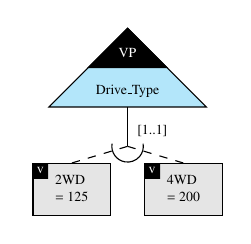
\begin{tikzpicture}
   \nodeVP{drivetype}{at={(0,0)}}{Drive\_Type};
   \nodeV{2wd}{below left=0.3cm of via_drivetype}{2WD}{= 125};
   \draw [dashed](via_drivetype)--(2wd.north);
   \nodeV{4wd}{below right=0.3cm of via_drivetype}{4WD}{= 200};
   \draw [dashed](via_drivetype)--(4wd.north);
  \end{tikzpicture}
 \end{center}

\vfill
\begin{exampleblock}{}
\begin{lstlisting}
  (1) { vp(VP,G) } :- vp_def(VP), group(G). 
  (2) 1 { v(V,G) : v_def(V,VP,_) } 1 :- vp(VP,G).
\end{lstlisting}
\end{exampleblock}
\vfill
\begin{itemize}
\item (1)
  各車種\code{G},各装備タイプ\code{VP}に対して,
  \code{G}が\code{VP}を装備することを意味するアトム
  \code{vp(VP,G)}を導入.
\item (2)
  各車種\code{G},各装備タイプ\code{VP}に対して,
  \code{vp(VP,G)}が成り立つならば,
  \code{G}が\code{VP}のオプション\code{V}を装備することを意味する
  アトム\code{v(V,G)}を導入し,そのうちの
  ちょうど1個を装備することを強制する.
\end{itemize}
\end{frame}
%%%%%%%%%%%%%%%%%%%%%%%%%%%%%%%%%%%%%%%%%%%%%%%%%%%%
\begin{frame}[fragile]{基本符号化: 燃費制約と目的関数}
\begin{exampleblock}{}\small
\begin{lstlisting}
  (3) iwr(S,G) :- 
         S = #sum { IWR,V : v(V,G), v_def(V,_,IWR) }, group(G).
  (4) fe(FE,G) :- iwr(S,G), fe_map(S,FE).
  (5) sv(SV,G) :- iwr(S,G), sv_map(S,SV).
  (6) :- not 0 #sum { (FE-t)*SV,FE,SV,G : fe(FE,G), sv(SV,G) }.
  (7) #maximize { SV,G : sv(SV,G) }.
\end{lstlisting}
\end{exampleblock}
\vfill
\begin{itemize}
\item (3)
  アトム\code{iwr(S,G)}は,車種\code{G}に実装されるオプションのIWR値の
  総和が\code{S}であることを表す.
\item (4--5)
  \code{fe(FE,G)}と\code{sv(SV,G)}は,
  それぞれ車種\code{G}の燃費が\code{FE},予想販売台数が\code{SV}
  であることを表す.
\item (6)
  CAFE方式の制約式を以下のように変形し,
  ASPの重み付き個数制約で表現している.ただし,$t$はCAFE基準値
  \[\sum_{i=1}^{n} (FE_{i}-t)\cdot SV_{i} \geq 0\]
\end{itemize}
\end{frame}
%%%%%%%%%%%%%%%%%%%%%%%%%%%%%%%%%%%%%%%%%%%%%%%%%%%%
\begin{frame}[fragile]{基本符号化の問題点}

\begin{exampleblock}{}\small
\begin{lstlisting}
  (3) iwr(S,G) :- 
         S = #sum { IWR,V : v(V,G), v_def(V,_,IWR) }, group(G).
\end{lstlisting}
\end{exampleblock}
\begin{itemize}
\item \code{(3)}で,IWR値の総和を表す項\code{S}の上下限は,
  \(
    0 \leq \texttt{S} \leq \sum_{j\in V}w_{j}
  \)
\item しかし,これは自明な上下限であり,各タイプが選択可能なオプション
  数の上下限値(今回はどちらも1),
  および,必須タイプかどうかの別を考慮することで,
  \alert{\bf \code{S}のドメインを縮小できる.}
\end{itemize}

\[
  \sum_{i\in VP^{*}}\min_{j\in V_{i}}w_{j}
  \leq \texttt{S} \leq
  \sum_{i\in VP}\max_{j\in V_{i}}w_{j}
\]

\begin{columns}\footnotesize
  \begin{column}{0.4\linewidth}
    \begin{itemize}
    \item $VP$:\ タイプの集合
    \item $VP*$:\ 必須なタイプの集合
    \item $V$:\ オプションの集合
    \end{itemize}
  \end{column}
  \begin{column}{0.45\linewidth}
    \begin{itemize}
    \item $V_i$:\ タイプ$i \in VP$ が選択可能なオプションの集合
    \item $w_j$:\ オプション$j \in V$ のIWR値
    \end{itemize}
  \end{column}
\end{columns}
\end{frame}
%%%%%%%%%%%%%%%%%%%%%%%%%%%%%%%%%%%%%%%%%%%%%%%%%%%%
\begin{frame}[fragile]{改良符号化}
\begin{exampleblock}{}
\footnotesize
\begin{lstlisting}
  (3') iwr(S,G) :- 
      S = #sum { IWR,V : v(V,G), v_def(V,_,IWR) },
      LB <= S, S <= UB, lb_iwr(LB), ub_iwr(UB), group(G).

  (10) ub_vp(UB,VP) :- UB = #max { IWR,V : v_def(V,VP,IWR) }, vp_def(VP).
  (11) lb_vp(LB,VP) :- LB = #min { IWR,V : v_def(V,VP,IWR) }, vp_def(VP).

  (12) ub_iwr(S) :- S = #sum { UB,VP : ub_vp(UB,VP) }.
  (13) lb_iwr(S) :- S = #sum { LB,VP : lb_vp(LB,VP), require_vp(VP) }.
\end{lstlisting}
\end{exampleblock}
 \begin{itemize}
 \item (10--11) 各装備タイプ\code{VP}に対して,選択可能な装備オプショ
   ンのIWR値の\structure{\bf 最大値\code{ub_vp(UB,VP)}}と\structure{\bf 最小値\code{lb_vp(LB,VP)}}を計算
 \item (12--13) IWR値の総和の\structure{\bf 上限値\code{ub_iwr(S)}}と\structure{\bf 下限値\code{lb_iwr(S)}}を計算
 \item この上下限を適用することで,基礎化後の(3')のルール数を抑えることができる.
 \end{itemize}
\end{frame}
%%%%%%%%%%%%%%%%%%%%%%%%%%%%%%%%%%%%%%%%%%%%%%%%%%%%
\begin{frame}[fragile]{拡張符号化}
 % \begin{block}{拡張符号化}
 %  予想販売台数の最大化に加えて,オプション数の最小化も可能にする.
 %  \begin{itemize}
 %   \item 製造ラインの削減や大量生産を促進することが狙い
 %  \end{itemize}  
 % \end{block}
 \begin{itemize}
  \item 製造ラインの削減や,大量生産を促進することを狙いとして,
	予想販売台数の最大化に加えて,オプション数の最小化も可能なように拡張
 \end{itemize}
 \begin{exampleblock}{}
  \begin{lstlisting}
   (7') #maximize { SV@2,G : sv(SV,G) }.

   (14) used_v(V) :- v(V,G).
   (15) #minimize { 1@1,V : used_v(V) }.
  \end{lstlisting}
 \end{exampleblock}
 \begin{itemize}
  \item アトム\scode{used_v(V)}は,オプション\code{V}がいずれかの装備仕様において
	実装されたことを意味する.
  \item 目的関数中の\code{@}の右側は優先度で,予想販売台数の最大化(優先度2),
	オプション数最小化(優先度1)の順に最適化される.
 \end{itemize}
\end{frame}
%%%%%%%%%%%%%%%%%%%%%%%%%%%%%%%%%%%%%%%%%%%%%%%%%%%%
\begin{frame}{最適解の全列挙 {\normalsize (CAFE基準値: 8.5km/L)}}
 \begin{exampleblock}{}
  \tiny
  \centering
    \begin{tabular}{l|l|c|c|c||c|c|c||c|c|c} 
    \multicolumn{2}{l|}{} & \multicolumn{3}{c||}{解1} & \multicolumn{3}{c||}{解2} & \multicolumn{3}{c}{\bf{解3}}\\ \hline
    \multicolumn{2}{l|}{装備仕様} & 1 & 2 & 3 & 1 & 2 & 3 & 1 & 2 & 3 \\ \hline
    装備 & \textsf{Grade}        & \textsf{STD}& \textsf{DX} & \textsf{LX}& \textsf{STD} & \textsf{DX}  & \textsf{LX}    & \textsf{STD} & \textsf{DX}  & \textsf{LX}       \\
        & \textsf{Drive\_Type}  & \textsf{4WD}  & \textsf{2WD} & \textsf{4WD} & \textsf{2WD} & \textsf{2WD} & \textsf{4WD} & \textsf{2WD} & \textsf{2WD} & \textsf{4WD}  \\
        & \textsf{Engine} & \textsf{V4} & \textsf{V6} & \textsf{V6} & \textsf{V6} & \textsf{V6} & \textsf{V6} & \textsf{V6} & \textsf{V6} & \textsf{V6}      \\ 
        & \textsf{Tire} & \textsf{16}	& \textsf{17} & \textsf{18} & \textsf{16}  & \textsf{17}  & \textsf{18} & \textsf{16} & \textsf{17} & \textsf{18} \\
        & \textsf{Transmission} & \textsf{5MT} & \textsf{HEV} & \textsf{10AT} & \textsf{CVT} & \textsf{HEV} & \textsf{10AT}  & \textsf{6AT} & \textsf{HEV} & \textsf{10AT}     \\
        & \textsf{Sun\_Roof} & \textsf{Panorama} & -   & -       & \textsf{Nomal} & -  & -     & -   & -   & -       \\ \hline
    \multicolumn{2}{l|}{IWR値の総和}  & 1,128 & 1,130   & 1,255    & 1,130 & 1,130&1,255  & 1,130& 1,130& 1,255     \\ %\hline
    \multicolumn{2}{l|}{燃費(km/L)}    & 8.9 & 8.8    & 8.0     & 8.8 & 8.8  & 8.0 & 8.8  & 8.8  & 8.0         \\ %\hline
    \multicolumn{2}{l|}{予想販売台数}  & 2,007  & 2,007   & 1,511   & 2,007 & 2,007 & 1,511 & 2,007& 2,007& 1,511       \\ \hline
    \multicolumn{2}{l|}{平均燃費(km/L)} & \multicolumn{3}{c||}{8.6} & \multicolumn{3}{c||}{8.5} & \multicolumn{3}{c}{8.5}\\ 
    \multicolumn{2}{l|}{予想販売台数(合計)}  & \multicolumn{3}{c||}{5,525} & \multicolumn{3}{c||}{5,525}  &\multicolumn{3}{c}{5,525}\\
    \multicolumn{2}{l|}{オプション数}  & \multicolumn{3}{c||}{14} & \multicolumn{3}{c||}{13}  &\multicolumn{3}{c}{12}\\ 
  \end{tabular}
 \end{exampleblock}
 \begin{itemize}
  \item 改良符号化では,予想販売台数が5,525台である最適解が(解1,解2,解3)の3つ存在する.
  \item 拡張符号化では,最適解はオプション数が最も小さい(解3)のただ1つだけとなる.
 \end{itemize}
 % \begin{alertblock}{}
 %  CAFE問題ソルバーでは,目的関数を柔軟に追加することにより,複数ある最適解に対して
 %  優劣をつけることができる.
 % \end{alertblock}
\end{frame}
%%%%%%%%%%%%%%%%%%%%%%%%%%%%%%%%%%%%%%%%%%%%%%%%%%%%
\begin{frame}{実行実験}
提案手法の有効性を評価するために,開発したCAFE問題ソルバーを用いた実行
実験を行なった.
\vfill
\begin{itemize}
\item ベンチマーク問題(計15問)
  \begin{itemize}
  \item 企業から提供された問題(3問)に対して
  \item 5通りのCAFE基準値$t\in\{8.5, 9.0, 9.5, 10.0, 10.5km/L\}$を適用
  \item 車種の数$n = 3$
  \end{itemize}
  \begin{exampleblock}\small
    \centering
    \begin{tabular}{ ll|r r r }
      問題名 & サイズ &  \#装備タイプ & \#装備オプション& \#依存制約\\ \hline
      small	 & 小規模   &   8 &   21  &   4	\\
      medium & 実用規模 &  86 &  226  & 147	\\
      big    & 大規模   & 315 & 1,337 &   0
    \end{tabular}
  \end{exampleblock}
\item ASPシステム: \textit{clingo-5.4.0}
\item 制限時間: 1問あたり2時間
\item 実験環境: Mac mini (3.2GHz, Intel Core i7, 64GB メモリ)
\end{itemize}
\end{frame}
%%%%%%%%%%%%%%%%%%%%%%%%%%%%%%%%%%%%%%%%%%%%%%%%%%%%
\begin{frame}{実験結果: 予想販売台数}
\begin{exampleblock}{}
  \centering
  \scriptsize
  \renewcommand{\arraystretch}{1.1}
  \tabcolsep = 7mm
  \begin{tabular}{l|r|rr}
  \lw{問題名} & CAFE  & \multicolumn{2}{c}{予想販売台数} \\ \cline{3-4}
              & 基準値 & 基本符号化 & 改良符号化 \\\hline    
   small & 8.5   & \alert{6,021*} & \alert{6,021*}       \\
   small & 9.0   & \alert{5,007*} & \alert{5,007*}       \\
   small & 9.5   & \alert{2,688*} & \alert{2,688*}       \\
   small & 10.0  & \alert{1,318*} & \alert{1,318*}       \\
   small & 10.5  & UNSAT          & UNSAT    \\\hline
   medium & 8.5  & 6,010          & \alert{6,021}        \\
   medium & 9.0  & \alert{5,595}  & \alert{5,595}        \\
   medium & 9.5  & \alert{3,447}  & 3,430        \\
   medium & 10.0 & 2,245          & \alert{2,250}        \\
   medium & 10.5 & 1,690          & \alert{1,845}        \\\hline
   big & 8.5     & -             & \alert{3,877}        \\
   big & 9.0     & 1,038          & \alert{4,623}        \\
   big & 9.5     & 688            & \alert{3,121}        \\
   big & 10.0    & 1,634          & \alert{2,064}        \\
   big & 10.5    & 538            & \alert{904}         \\\hline
   \multicolumn{2}{l}{最適値・最良値の数} & \multicolumn{1}{r}{6} & \alert{13} \\
  \end{tabular}
\end{exampleblock}
\vfill
\begin{itemize}%\small
\item 改良符号化が,より多くの問題に対して優れた結果を示した.
\item 特に,大規模な問題に対する改良符号化の優位性が確認できた.
 \end{itemize}	
\end{frame}
%%%%%%%%%%%%%%%%%%%%%%%%%%%%%%%%%%%%%%%%%%%%%%%%%%%%
\begin{frame}{実験結果: 最適解を求めるまでのCPU時間}
  
\begin{exampleblock}{}\centering 
  \renewcommand{\arraystretch}{1.2}
  \tabcolsep = 4mm
  \begin{tabular}{cc|r|rr}
    \lw{問題名} & \lw{結果} & CAFE  & \multicolumn{2}{c}{CPU時間(秒)} \\ \cline{4-5}
             &  & 基準値 & 基本符号化 & 改良符号化 \\\hline
    small  & OPT &  8.5  & 37.868         & \alert{23.318}  \\
    small  & OPT &  9.0  & 48.965         & \alert{43.362}  \\
    small  & OPT &  9.5  & \alert{95.110} & 173.172         \\
    small  & OPT & 10.0  & 99.954         & \alert{0.343}   \\
    small  & UNSAT   & 10.5  & 439.613    & \alert{0.080}   \\\hline
   \multicolumn{3}{r}{平均}  & 144.302     & \alert{48.055}
  \end{tabular}
\end{exampleblock}
\begin{itemize}
\item 5問中4問に対して,改良符号化がより高速に解を求めている.
%\item 平均では,改良符号化のCPU時間は基本符号化の約1/3であった.
\end{itemize}
\end{frame}
%%%%%%%%%%%%%%%%%%%%%%%%%%%%%%%%%%%%%%%%%%%%%%%%%%%%
\begin{frame}{車種の数を増やした実験}
 \begin{exampleblock}{}\centering 
  \renewcommand{\arraystretch}{1.1}
  \tabcolsep = 4mm
  \scriptsize
  \begin{tabular}{cr|c|rr}
    \lw{車種の数($n$)} & CAFE  & \lw{結果} & \multicolumn{2}{c}{CPU時間(秒)} \\ \cline{4-5}
                      & 基準値 &          &  基本符号化      & 改良符号化 \\\hline
   3 & 8.5   & \alert{OPT}       & 48.126          & 34.442          \\
   3 & 9.0   & \alert{OPT}       & 25.648          & 12.837          \\
   3 & 9.5   & \alert{OPT}       & 26.223          & 49.161          \\
   3 & 10.0  & \alert{OPT}       & 447.674         & 0.394           \\
   3 & 10.5  & \structure{UNSAT}     & 1103.135        & 0.085           \\\hline 
   6 & 8.5   & SAT       & TO        & TO        \\
   6 & 9.0   & \alert{OPT}       & 1386.491        & 1509.845        \\
   6 & 9.5   & \alert{OPT}       & 532.665         & TO        \\
   6 & 10.0  & \structure{UNSAT}     & TO        & 1.670           \\
   6 & 10.5  & \structure{UNSAT}     & 599.330         & 0.134           \\\hline
   12 & 8.5  & SAT       & TO        & TO        \\
   12 & 9.0  & SAT       & TO        & TO        \\
   12 & 9.5  & \structure{UNSAT}     & 1540.594        & 519.988         \\
   12 & 10.0 & \structure{UNSAT}     & 641.738         & 33.014          \\
   12 & 10.5 & \structure{UNSAT}     & 6.117           & 0.483           \\
  \end{tabular}
 \end{exampleblock}
 \begin{itemize}
  \scriptsize
  \item $n=3$では5問すべて,$n=6$では5問中4問について、最適解あるいはUNSATを求めることができた.
  \item $n=12$では5問中3問はUNSATで,残り2問いついては実行可能解は得られたが,
	その最適性を証明するには至らなかった.
 \end{itemize}
\end{frame}
%%%%%%%%%%%%%%%%%%%%%%%%%%%%%%%%%%%%%%%%%%%%%%%%%%%%
\begin{frame}{まとめ}
 解集合プログラミング(ASP)を用いたCAFE問題ソルバーの設計・実装
 について述べた.
 \begin{alertblock}{開発したCAFE問題ソルバーの特長}
  \begin{itemize}
   \item \structure{\bf 記述性: }
	 ASPの表現力の高さを活かし,CAFE問題の制約を簡潔に記述できる.
   \item \structure{\bf 効率性: }
	 改良符号化を用いることで,大規模な問題にも適用可能である.
   \item \structure{\bf 拡張性: }
	 装備オプション数の最小化など,ユーザの選好にあわせて目的関数を柔軟に
	 追加できる.
  \end{itemize}
 \end{alertblock} 
\vfill
\begin{small}
\begin{block}{今後の課題}
\begin{itemize}
\item 装備に関する制約は,まず企画部門で設定され,開発部門,生産部門,
  販売部門に受け渡され,各部門で制約が追加されながら徐々に成
  熟していく.
\item これら様々な制約を実装することにより,CAFE問題ソルバーを拡張する
  ことが今後の課題である.
\end{itemize}
\end{block}
\end{small}
\end{frame}
%%%%%%%%%%%%%%%%%%%%%%%%%%%%%%%%%%%%%%%%%%%%%%%%%%%% 
\begin{frame}{質問リスト}
 \begin{itemize}
  \item 制約について
	\begin{itemize}
	 \item 範囲制約,要求制約,CAFE制約以外の制約はありますか?
	 \item エンジンなどのオプションによって燃費のテーブルが
	       変わることはありますか?
	\end{itemize}
  \item 目的関数について
	\begin{itemize}
	 \item 販売台数最大化,装備オプション数最小化以外にありますか?
	 \item オプション数最小化をする場合,各オプションの重み(IWR?)を
	       考慮する必要はありますか?
	\end{itemize}
  \item 現場での装備仕様決定の現状について
	\begin{itemize}
	 \item 車両装備仕様のコスト(人員・費用・時間)について知りたいです.
	 \item 仕様決定までの全体の流れを知りたいです.
	 \item 販売台数はどうやって予想していますか?
	 \item 現状扱っている問題のサイズ(タイプ,オプション,
	       車種の数など)はどの程度ですか?
	\end{itemize}
 \end{itemize}
\end{frame}
%%%%%%%%%%%%%%%%%%%%%%%%%%%%%%%%%%%%%%%%%%%%%%%%%%%% 
\begin{frame}{}
  \vskip 3em
  \begin{center}\LARGE
    ご清聴ありがとうございました.    
  \end{center}
\end{frame}
%%%%%%%%%%%%%%%%%%%%%%%%%%%%%%%%%%%%%%%%%%%%%%%%%%%% 
\appendix
\backupbegin
%%%%%%%%%%%%%%%%%%%%%%%%%%%%%%%%%%%%%%%%%%%%%%%%%%%%
% \begin{frame}[fragile]{IWR値の上下限}
%  \begin{exampleblock}{}
%   \footnotesize
%   \begin{lstlisting}
%    ub_vp(UB,VP) :- UB = #max { IWR,V : v_def(V,VP,IWR) }, vp_def(VP).
%    lb_vp(LB,VP) :- LB = #min { IWR,V : v_def(V,VP,IWR) }, vp_def(VP).

%    ub_iwr(S) :- S = #sum { UB,VP : ub_vp(UB,VP) }.
%    lb_iwr(S) :- S = #sum { LB,VP : lb_vp(LB,VP), require_vp(VP) }.
%   \end{lstlisting}
%  \end{exampleblock}
%  \begin{itemize}
%   \item アトム\scode{ub_vp(UB,VP)}, \scode{lb_vp(LB,VP)}は,
% 	タイプ\code{VP}に属するオプションの中で最大のIWR値が\code{UB},
% 	最小のIWR値が\code{LB}であることを表す.
%   \item アトム\scode{ub_iwr(S)}は,すべての\code{VP}についての
% 	\code{UB}の和が\code{S}であることを表す.
%   \item アトム\scode{lb_iwr(S)}は,必須タイプである\code{VP}についての
% 	\code{LB}の和が\code{S}であることを表す.
%  \end{itemize}
% \end{frame}
%%%%%%%%%%%%%%%%%%%%%%%%%%%%%%%%%%%%%%%%%%%%%%%%%%%%
\begin{frame}{基礎化後のルール数}
 \begin{exampleblock}{}\centering 
  \renewcommand{\arraystretch}{1.2}
  \tabcolsep = 4mm
  \begin{tabular}{crr} 
   問題名    & 基本符号化       & 改良符号化    \\ \hline
   small    &  83,520 (1.00)  & 32,855 (0.39) \\ 
   medium   &  93,017 (1.00)  & 56,940 (0.61) \\
   big	    & 155,654 (1.00)  & 42,190 (0.27) \\ 
  \end{tabular}
 \end{exampleblock}
 \begin{itemize}
  \item 改良符号化は,基本符号化と比較して,基礎化後のルール数を
	少なく抑えられている.
  \item 特にbigでは,70\%以上のルール数の削減に成功している.
 \end{itemize}
 % \begin{alertblock}{}
 %  このルール数の削減が,改良符号化の大規模問題に対する優位性につながっていると考えられる.
 % \end{alertblock}
\end{frame}
%%%%%%%%%%%%%%%%%%%%%%%%%%%%%%%%%%%%%%%%%%%%%%%%%%%%
\begin{frame}[fragile]{基本符号化: 依存制約(要求・排他)}
 \begin{center} 
 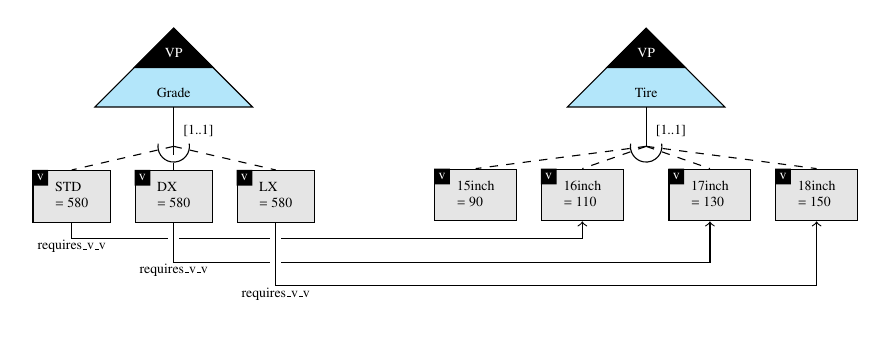
\begin{tikzpicture}
 % Grade
  \nodeVP{grade}{at={(0,0)}}{Grade};
  \nodeV{dx}{below=0.3cm of via_grade}{DX}{= 580};
  \draw[dashed](via_grade)--(dx.north);
  \nodeV{std}{left=0.3cm of dx}{STD}{= 580};
  \draw[dashed](via_grade)--(std.north);
  \nodeV{lx}{right=0.3cm of dx}{LX}{= 580};
  \draw[dashed](via_grade)--(lx.north);

  % Tire
  \nodeVP{tire}{right=6cm of grade}{Tire};
  \nodeV{16inch}{below left=0.4cm of via_tire}{16inch}{= 110};
  \nodeV{17inch}{below right=0.4cm of via_tire}{17inch}{= 130};
  \nodeV{15inch}{left=0.3cm of 16inch}{15inch}{= 90};
  \nodeV{18inch}{right=0.3cm of 17inch}{18inch}{= 150};
  \draw [dashed](via_tire)--(15inch.north);
  \draw [dashed](via_tire)--(16inch.north);
  \draw [dashed](via_tire)--(17inch.north);
  \draw [dashed](via_tire)--(18inch.north);

  % require
  \draw[->] (std.south)--++(0,-0.2) node[below=-1mm] {\tiny{requires\_v\_v}} -|(16inch.south);
  \draw[white,line width=4pt](dx.south) ++(0,-0.1)--++(0,-0.5);
  \draw[->] (dx.south)--++(0,-0.5) node[below=-1mm] {\tiny{requires\_v\_v}} -|(17inch.south);
  \draw[white,line width=4pt] (lx.south) ++(0,-0.1)--++(0,-0.8);
  \draw[->] (lx.south)--++(0,-0.8) node[below=-1mm] {\tiny{requires\_v\_v}} -|(18inch.south);
 \end{tikzpicture}
 \end{center}

\vfill
\begin{exampleblock}{}
\begin{lstlisting}
  (8) :- require_v_v(V1,V2), v(V1,G), not v(V2,G).
  (9) :- exclude_v_v(V1,V2), v(V1,G), v(V2,G).
\end{lstlisting}
\end{exampleblock}
\vfill
\begin{itemize}
\item (8)
  要求関係\code{require_v_v(V1,V2)}が与えられたとき,
  車種\code{G}がオプション\code{V1}を実装するならば,
  \code{G}は\code{V2}も実装しなければならない.
\item (9)
  排他関係\code{exclude_v_v(V1,V2)}が与えられたとき,
  車種\code{G}が\code{V1}と\code{V2}を
  同時に実装することはない.
\end{itemize}
\end{frame}


%%%%%%%%%%%%%%%%%%%%%%%%%%%%%%%%%%%%%%%%%%%%%%%%%%%%
\backupend
\end{document}

%%% Local Variables:
%%% mode: japanese-latex
%%% TeX-master: t
%%% End:
